%% For double-blind review submission, w/o CCS and ACM Reference (max submission space)
\documentclass[sigplan]{acmart}\settopmatter{printfolios=true,printccs=false,printacmref=false}
%\settopmatter{authorsperrow=2}
%% For double-blind review submission, w/ CCS and ACM Reference
%\documentclass[sigplan,review,anonymous]{acmart}\settopmatter{printfolios=true}
%% For single-blind review submission, w/o CCS and ACM Reference (max submission space)
%\documentclass[sigplan,review]{acmart}\settopmatter{printfolios=true,printccs=false,printacmref=false}
%% For single-blind review submission, w/ CCS and ACM Reference
%\documentclass[sigplan,review]{acmart}\settopmatter{printfolios=true}
%% For final camera-ready submission, w/ required CCS and ACM Reference
%\documentclass[sigplan]{acmart}\settopmatter{}


%% Conference information
%% Supplied to authors by publisher for camera-ready submission;
%% use defaults for review submission.
\acmConference[]{Project Report}{June 18, 2019}{Runtime Verification, Inc.}
\acmYear{2019}
\acmISBN{} % \acmISBN{978-x-xxxx-xxxx-x/YY/MM}
\acmDOI{} % \acmDOI{10.1145/nnnnnnn.nnnnnnn}
\startPage{1}

%% Copyright information
%% Supplied to authors (based on authors' rights management selection;
%% see authors.acm.org) by publisher for camera-ready submission;
%% use 'none' for review submission.
\setcopyright{none}
%\setcopyright{acmcopyright}
%\setcopyright{acmlicensed}
%\setcopyright{rightsretained}
%\copyrightyear{2018}           %% If different from \acmYear

%% Bibliography style
\bibliographystyle{ACM-Reference-Format}
%% Citation style
%\citestyle{acmauthoryear}  %% For author/year citations
%\citestyle{acmnumeric}     %% For numeric citations
%\setcitestyle{nosort}      %% With 'acmnumeric', to disable automatic
                            %% sorting of references within a single citation;
                            %% e.g., \cite{Smith99,Carpenter05,Baker12}
                            %% rendered as [14,5,2] rather than [2,5,14].
%\setcitesyle{nocompress}   %% With 'acmnumeric', to disable automatic
                            %% compression of sequential references within a
                            %% single citation;
                            %% e.g., \cite{Baker12,Baker14,Baker16}
                            %% rendered as [2,3,4] rather than [2-4].


%%%%%%%%%%%%%%%%%%%%%%%%%%%%%%%%%%%%%%%%%%%%%%%%%%%%%%%%%%%%%%%%%%%%%%
%% Note: Authors migrating a paper from traditional SIGPLAN
%% proceedings format to PACMPL format must update the
%% '\documentclass' and topmatter commands above; see
%% 'acmart-pacmpl-template.tex'.
%%%%%%%%%%%%%%%%%%%%%%%%%%%%%%%%%%%%%%%%%%%%%%%%%%%%%%%%%%%%%%%%%%%%%%


%% Some recommended packages.
\usepackage{booktabs}   %% For formal tables:
                        %% http://ctan.org/pkg/booktabs
\usepackage{subcaption} %% For complex figures with subfigures/subcaptions
                        %% http://ctan.org/pkg/subcaption

\usepackage{listings}
\usepackage{tikz}
\usetikzlibrary{positioning}
\usetikzlibrary{graphs}
\usepackage{balance}

% colors
\definecolor{shadecolor}{gray}{1.00}
\definecolor{darkgray}{gray}{0.30}
\definecolor{violet}{rgb}{0.56, 0.0, 1.0}
\definecolor{forestgreen}{rgb}{0.13, 0.55, 0.13}

% Col language definition
\lstdefinelanguage{Coq} {
mathescape=true,						
texcl=false,
morekeywords=[1]{
  Add,
  All,
  Arguments,
  Axiom,
  Bind,
  Canonical,
  Check,
  Close,
  CoFixpoint,
  CoInductive,
  Coercion,
  Contextual,
  Corollary,
  Defined,
  Definition,
  Delimit,
  End,
  Example,
  Export,
  Fact,
  Fixpoint,
  Goal,
  Graph,
  Hint,
  Hypotheses,
  Hypothesis,
  Implicit,
  Implicits,
  Import,
  Inductive,
  Lemma,
  Let,
  Local,
  Locate,
  Ltac,
  Maximal
  Module,
  Morphism,
  Next,
  Notation,
  Obligation,
  Open,
  Parameter,
  Parameters,
  Prenex,
  Print,
  Printing,
  Program,
  Projections,
  Proof,
  Proposition,
  Qed,
  Record,
  Relation,
  Remark,
  Require,
  Reserved,
  Resolve,
  Rewrite,
  Save,
  Scope,
  Search,
  Section,
  Show,
  Strict,
  Structure,
  Tactic,
  Theorem,
  Unset,
  Variable,
  Variables,
  View,
  inside,
  outside
},
morekeywords=[2]{
  as,
  cofix,
  else,
  end,
  exists,
  exists2,
  fix,
  for,
  forall,
  fun,
  if,
%  in,
  is,
  let,
  match,
  nosimpl,
  of,
  return,
  struct,
  then,
  vfun,
  with
},
morekeywords=[3]{Type, Prop, Set, True, False},
morekeywords=[4]{
  after,
  apply,
  assert,
  auto,
  bool_congr,
  case,
  change,
  clear,
  compute,
  congr,
  cut,
  cutrewrite,
  destruct,
  elim,
  field,
  fold,
  generalize,
  have,
  heval, 
  hnf,
  induction,
  injection,
  intro,
  intros,
  intuition,
  inversion,
  left,
  loss,
  move,
  nat_congr,
  nat_norm,
  pattern,
  pose,
  refine,
  rename,
  replace,
  revert,
  rewrite,
  right,
  ring,
%  set,
  simpl,
  split,
  suff,
  suffices,
  symmetry,
  transitivity,
  trivial,
  unfold,
  unlock,
  using,
  without,
  wlog,
  autorewrite
},        
morekeywords=[5]{
  assumption,
  by,
  contradiction,
  done,
  exact,
  lia,
  gappa,
  omega,
  reflexivity,
  romega,
  solve,
  tauto,
  discriminate,
  unsat
},
morecomment=[s]{(*}{*)},
morekeywords=[6]{do, first, try, idtac, repeat},
showstringspaces=false,
morestring=[b]",
% Size of tabulations
tabsize=3,							
% Enables ASCII chars 128 to 255
extendedchars=true,  		 		
% Case sensitivity
sensitive=true, 
% Automatic breaking of long lines
breaklines=false,
% Default style fors listings
%basicstyle=\scriptsize\ttfamily,
basicstyle=\footnotesize\ttfamily,
% Position of captions is bottom
captionpos=b,							
% Full flexible columns 
columns=[l]fullflexible,
% Style for (listings') identifiers
identifierstyle={\color{black}},
% Style for declaration keywords
keywordstyle=[1]{\color{violet}},
% Style for gallina keywords
keywordstyle=[2]{\color{forestgreen}},
% Style for sorts keywords
keywordstyle=[3]{\color{forestgreen}},
% Style for tactics keywords
keywordstyle=[4]{\color{blue}},
% Style for terminators keywords
keywordstyle=[5]{\color{red}},
%Style for iterators
keywordstyle=[6]{\color{violet}},
% Style for strings
stringstyle=,
% Style for comments
commentstyle=\it\ttfamily\color{brown},
% Style for lines numbering
numberstyle=\tiny,
literate={\\/}{{$\lor~$}}1
         {/\\}{{$\land~$}}1
         {<>}{{$\neq~$}}1
         {:->}{{$\mapsto~$\!}}1
         {\\->}{{$\mapsto~$\!}}1
         {<--}{{$\asgn~$}}1
         {\\in}{{$\in~$}}1
         {\\notin}{{$\notin~$}}1
         {++}{{$+\!+\!~$}}1
         {->}{{$\to~$}}1
         {forall}{{$\forall~$}}1
         {exists}{{$\exists~$}}1
         {=>}{{$\Rightarrow~$}}1
         {\\~}{{$\lnot\;$}}1
%         {\\+}{{$\!\join\!~$}}1
}

\lstdefinestyle{Coq}{language=Coq}
\lstset{language=Coq}


\begin{document}

%% Title information
\title[Modeling and Verification of the Algorand Consensus Protocol]{Modeling and Verification of the\\ Algorand Consensus Protocol}
                                        %% when present, will be used in
                                        %% header instead of Full Title.
%\titlenote{with title note}             %% \titlenote is optional;
                                        %% can be repeated if necessary;
                                        %% contents suppressed with 'anonymous'
%\subtitle{Subtitle}                     %% \subtitle is optional
%\subtitlenote{with subtitle note}       %% \subtitlenote is optional;
                                        %% can be repeated if necessary;
                                        %% contents suppressed with 'anonymous'


%% Author information
%% Contents and number of authors suppressed with 'anonymous'.
%% Each author should be introduced by \author, followed by
%% \authornote (optional), \orcid (optional), \affiliation, and
%% \email.
%% An author may have multiple affiliations and/or emails; repeat the
%% appropriate command.
%% Many elements are not rendered, but should be provided for metadata
%% extraction tools.

%% Authors
\author{Musab A. Alturki}
\affiliation{
  %\position{Position1}
  %\department{Department1}              %% \department is recommended
  \institution{Runtime Verification, Inc.}            %% \institution is required
  %\streetaddress{Street1 Address1}
  %\city{City1}
  %\state{State1}
  %\postcode{Post-Code1}
  %\country{USA}                    %% \country is recommended
}
%\email{musab.alturki@runtimeverification.com}          %% \email is recommended
\affiliation{
  %\position{Position1}
  %\department{Department1}              %% \department is recommended
  \institution{King Fahd University of Petroleum and Minerals}            %% \institution is required
  %\streetaddress{Street1 Address1}
  %\city{City1}
  %\state{State1}
  %\postcode{Post-Code1}
  %\country{USA}                    %% \country is recommended
}
\email{musab@kfupm.edu.sa}          %% \email is recommended

\author{Brandon Moore}
\affiliation{
  %\position{Position1}
  %\department{Department1}              %% \department is recommended
  \institution{Runtime Verification, Inc.}            %% \institution is required
  %\streetaddress{Street1 Address1}
  %\city{City1}
  %\state{State1}
  %\postcode{Post-Code1}
  %\country{USA}                    %% \country is recommended
}
\email{brandon.moore@runtimeverification.com}          %% \email is recommended

\author{Karl Palmskog}
%\authornote{with author1 note}          %% \authornote is optional;
%                                       %% can be repeated if necessary
%\orcid{nnnn-nnnn-nnnn-nnnn}             %% \orcid is optional
\affiliation{
  %\position{Position1}
  %\department{Department1}              %% \department is recommended
  \institution{The University of Texas at Austin}            %% \institution is required
  %\streetaddress{Street1 Address1}
  %\city{City1}
  %\state{State1}
  %\postcode{Post-Code1}
  %\country{USA}                    %% \country is recommended
}
\email{palmskog@acm.org}          %% \email is recommended

%% Author with single affiliation.
\author{Lucas Pe{\~n}a}
%\authornote{with author1 note}          %% \authornote is optional;
                                        %% can be repeated if necessary
%\orcid{nnnn-nnnn-nnnn-nnnn}             %% \orcid is optional
\affiliation{
  %\position{Position1}
  %\department{Department1}              %% \department is recommended
  \institution{Runtime Verification, Inc.}            %% \institution is required
  %\streetaddress{Street1 Address1}
  %\city{City1}
  %\state{State1}
  %\postcode{Post-Code1}
  %\country{USA}                    %% \country is recommended
}
%\email{lucas.pena@runtimeverification.com}          %% \email is recommended
\affiliation{
  %\position{Position1}
  %\department{Department1}              %% \department is recommended
  \institution{University~of~Illinois~at~Urbana-Champaign}            %% \institution is required
  %\streetaddress{Street1 Address1}
  %\city{City1}
  %\state{State1}
  %\postcode{Post-Code1}
  %\country{USA}                    %% \country is recommended
}
\email{lpena7@illinois.edu}          %% \email is recommended

\author{Grigore Ro{\c s}u}
\affiliation{
  %\position{Position1}
  %\department{Department1}              %% \department is recommended
  \institution{Runtime Verification, Inc.}            %% \institution is required
  %\streetaddress{Street1 Address1}
  %\city{City1}
  %\state{State1}
  %\postcode{Post-Code1}
  %\country{USA}                    %% \country is recommended
}
%\email{grigore.rosu@runtimeverification.com}          %% \email is recommended
\affiliation{
  %\position{Position1}
  %\department{Department1}              %% \department is recommended
  \institution{University of Illinois at Urbana-Champaign}            %% \institution is required
  %\streetaddress{Street1 Address1}
  %\city{City1}
  %\state{State1}
  %\postcode{Post-Code1}
  %\country{USA}                    %% \country is recommended
}
\email{grosu@illinois.edu}          %% \email is recommended

%\shortauthors{Palmskog, Gligoric, Pe{\~n}a, and Ro{\c s}u}

%% Abstract
%% Note: \begin{abstract}...\end{abstract} environment must come
%% before \maketitle command
\begin{abstract}
The Algorand consensus protocol is at the core of the Algorand platform for secure and decentralized digital currencies and transactions. In this report, we describe our effort to model and formally verify the Algorand consensus protocol in the Coq proof assistant. We give an overview of the protocol, outline our model of the protocol as a state transition system, and describe how its properties are formalized and proved. A key contribution of this work is the elucidation of the assumptions under which the main safety property of the protocol holds. The Coq source files are available at:\\
\url{https://github.com/runtimeverification/algorand-verification}
\end{abstract}


%% 2012 ACM Computing Classification System (CSS) concepts
%% Generate at 'http://dl.acm.org/ccs/ccs.cfm'.
%\begin{CCSXML}
%<ccs2012>
%<concept>
%<concept_id>10011007.10011006.10011008</concept_id>
%<concept_desc>Software and its engineering~General programming languages</concept_desc>
%<concept_significance>500</concept_significance>
%</concept>
%<concept>
%<concept_id>10003456.10003457.10003521.10003525</concept_id>
%<concept_desc>Social and professional topics~History of programming languages</concept_desc>
%<concept_significance>300</concept_significance>
%</concept>
%</ccs2012>
%\end{CCSXML}

%\ccsdesc[500]{Software and its engineering~General programming languages}
%\ccsdesc[300]{Social and professional topics~History of programming languages}
%% End of generated code


%% Keywords
%% comma separated list
%\keywords{keyword1, keyword2, keyword3}  %% \keywords are mandatory in final camera-ready submission

%% \maketitle
%% Note: \maketitle command must come after title commands, author
%% commands, abstract environment, Computing Classification System
%% environment and commands, and keywords command.
\maketitle
\renewcommand{\shortauthors}{M. A. Alturki, B. Moore, K. Palmskog, L. Pe{\~n}a, and G. Ro{\c s}u}

\section{Introduction}

Algorand is a platform for secure and decentralized digital currencies and transactions~\cite{Micali2019}. At the core of the Algorand platform is the Algorand consensus protocol~\cite{Chen2018,Chen2019}, a pure Proof-of-Stake (PoS) protocol that provides efficient, secure, and scalable operation while remaining decentralized. The basic idea in pure PoS is to make the security of the system dependent only on how honest the majority of its asset owners are, without having to rely on any specific subset of participants or having to lock up assets and penalize users.

Distributed consensus protocols are complex, and subject to general limitations even in non-adversarial settings~\cite{Fischer1985}. They typically involve interaction between many independent and potentially untrusted nodes in a large network where asynchronous and failure-prone communication is the norm rather than the exception.
Algorand, in particular, specifies not only the node-local behavior, but also deals with message propagation and delivery, to be able to address two types of attacks: (1) attacks that corrupt participating nodes so that they no longer follow the protocol, e.g., to produce fake transactions or to cast votes for the wrong transactions, and (2) attacks on the underlying network in which the system is deployed, for instance by intercepting, manipulating, and delaying messages. When an attacker gains full control of message delivery in a network, the network is said to be partitioned. Unlike Algorand, most existing consensus protocols do not consider what happens when a network is partitioned or after the network recovers from a partition.

Consensus systems are now the backbone of large cryptocurrencies worth billions of US dollars. This means that vulnerabilities can have catastrophic consequences. Consequently, ensuring correctness and resilience against malicious behavior while designing a consensus protocol is an important and challenging task. Having strong guarantees of correctness and developing a thorough understanding of protocol assumptions can significantly reduce the risk of catastrophic events.

In this report, we describe our effort to model and verify the Algorand consensus protocol using deductive verification. In this approach, systems are modeled and specified inside expressive formal logical systems, and verified in a similar way to how mathematicians prove theorems - in principle by elaborating proofs of statements step-by-step. In the spectrum of formal verification techniques, deductive verification provides the strongest guarantees, and thus the highest degree of trustworthiness, but at the expense of being the most demanding. Specifically, we use the Coq proof assistant~\cite{CoqArt}, a tool based on type theory developed for more than 30 years and used in several large-scale verification projects~\cite{Leroy2009,Woos2016}.

We developed a model of Algorand consensus in Coq in the form of a \emph{transition system}, over which we stated and ultimately proved the \emph{asynchronous safety} property: no two honest nodes certify two different blocks, even when the adversary has complete control of message delivery in the network. We also precisely pin down the assumptions under which the safety theorem holds. Beyond the safety theorem, we intend for this formalization to lay the foundation for further modeling and verification efforts related to the Algorand consensus protocol.

%Coq is developed for more than 30 years and very well supported. Coq has previously been used to develop a verified C compiler, formally prove mathematical results such as the four-color theorem, and verify distributed protocols (see, for example, our previous Casper formal verification effort for the Ethereum Foundation).

%We developed a model of the Algorand consensus protocol in Coq, a proof assistant based on type theory~\cite{}

%and proved a slew of its properties that we then used to ultimately show the asynchronous safety property: no two honest nodes certify two different blocks, even when the adversary has complete control of message delivery in the network.

%This report describes our effort to model the protocol and specify and verify its properties. Moreover, we describe the formalization of the assumptions under which the safety theorem holds. Beyond the safety theorem, we intend for this formalization in Coq to lay the foundation for further future modeling and verification efforts of the Algorand consensus protocol.

%A key characteristic of Algorand is that it almost never forks. Forking happens when consensus on a single block for a round is not reached and multiple candidate blocks are available for that round. Having different subsets of nodes decide on appending different blocks to the chain means that transactions appearing in these conflicting blocks are not finalized since only one of these blocks will eventually belong to the canonical chain, the chain that is deemed most accepted by the nodes (there are different methods for deciding the canonical chain, e.g. the longest chain in Bitcoin). Algorand avoids this problem by design: at most one block can receive the majority of votes in a round. This property implies that once a block of transactions appear in the chain, they can immediately be considered final. This has the potential of allowing extremely high levels of scalability. This no-forking property is referred to as Asynchronous safety, which states that no two honest nodes will certify two different blocks, even when the adversary has complete control of message delivery in the network. 

\section{Background}
\label{sec:background}
This section generally introduces blockchain and consensus protocols, gives an overview of Algorand, and provides the pertinent Coq background.

\subsection{Blockchains and Consensus Protocols}

A blockchain is an ordered sequence of cryptographically linked blocks of records, in much the same way as links in a chain are firmly latched in sequence. A blockchain provides a persistent, tamper-proof and globally accessible ledger of transactions. It is built using well-established and publicly known cryptographic tools, including most importantly one-way hash functions. Anyone can verify the validity of its transactions, and no one can tamper with a transaction or claim a transaction exists that does not appear in the chain.

This makes blockchains particularly well suited for building self-governing and autonomous distributed systems. Indeed, a blockchain is a key component for allowing a collection of nodes in a communication network (who do not necessarily trust each other) to work collectively and make decentralized decisions. Nevertheless, the nodes will need more than just a blockchain to achieve proper decentralized operation. Specifically, they need a mechanism for identifying and agreeing on the next block of transactions to be appended to the chain, a mechanism known as a consensus protocol.

A consensus protocol typically proceeds in rounds, where the objective of a round is to produce the next block and record it in the chain. As such, a consensus protocol includes both:
(1) a mechanism for decentralized selection of one or more block proposers or producers of a round in the protocol, and 
(2) a mechanism for achieving decentralized consensus on a single block to be appended to the chain. 

In an idealistic (and rather unrealistic) setup, in which communication networks are perfectly reliable with zero-delay message delivery, and in which all participating nodes run error-free code and behave honestly, achieving consensus on a single block in each round is a trivial task. All nodes would instantaneously see all proposed blocks and their trusted opinions about them. In reality, however, the situation is very different. Distributed systems utilize global Internet (IP-based) communication networks, which are inherently unreliable and where significant message transmission delays are not uncommon. Furthermore, nodes may deviate from the protocol, either intentionally (when compromised by malicious users) or unintentionally (due to internal errors). These complications can hinder the consensus process, resulting potentially in the system being unusable or in losing large amounts of assets maintained by the system.

Therefore, consensus protocols need to maintain a consistent global view of the system while relying only on the local knowledge at the level of its individual (honest) nodes. Moreover, these protocols must ensure continuous and fair operation of the system in the presence of both benign node or network failures and maliciously behaving nodes. Consequently, consensus protocols are inherently complex, consisting of multiple asynchronous steps and utilizing a wealth of cryptographic and randomization schemes, and possibly some economic incentive structures, whose goal is to reward compliant behaviors and penalize deviations from the protocol.

A class of consensus protocols, pioneered by Bitcoin~\cite{Nakamoto2008} and referred to as Proof-of-Work (PoW), achieves consensus primarily through a process called mining, in which all participating nodes in the network compete on solving complex cryptographic puzzles to produce and record blocks. Although it provided workable solutions to the decentralized consensus challenge, PoW is now widely known to suffer from efficiency, scalability, and security problems. The mining process is inherently computationally expensive, slow, and wasteful, resulting in wasting significant amounts of energy while imposing high transaction fees. Furthermore, PoW tends in practice to result in centralized systems, in which the bulk of the mining power (and hence the power of deciding the fate of the blockchain) falls in the hands of a small subset of users: those who can afford to invest in very powerful computing resources, or who can simply join forces in mining pools. Centralization defeats the purpose of the protocol and poses a major security concern: those who control the majority of the mining power need to be trusted, and even if they are, they make the system a much easier target for attacks.

An alternative mechanism that promises to alleviate these problems is Proof-of-Stake (PoS), in which the burden of producing blocks and selecting the next block to augment the blockchain is placed on a suitably selected subset of nodes (typically much smaller than the entire set of participating nodes), called a committee. In some variations of PoS, called delegated PoS, the committee is trusted and is usually fixed. In other variations, generally referred to as bonded PoS, participation in a committee requires staking some of the blockchain's underlying cryptographic assets (such as cryptocurrency or tokens), or locking up these assets for an extended period of time so that they cannot be expended or moved. The stake of a committee member (relative to the total stake in the system) determines the member's voting power when deciding the next block for a given round in the protocol. Furthermore, a node's stake can also be used as collateral to be (fully or partially) reclaimed by the system if a node is found to misbehave.

However, many important questions arise when designing a PoS protocol. How is the committee selected? One would want to have a selection process that is fair and representative, and hard to manipulate by a malicious user. Moreover, a committee that is fixed for a prolonged period of time can be easily attacked and presents a potential single point-of-failure for the system. But how often should the committee be changed? What is a suitable size of the committee in relation to the total population of nodes in the network? How should the voting process be designed? These and other design choices can significantly affect the efficiency, scalability and security of a PoS blockchain system. 

\subsection{Overview of Algorand}

We highlight below some of Algorand's unique features. More detailed descriptions of these features and others are available elsewhere~\cite{Chen2018,Chen2019}.

Algorand almost never forks. Forking happens when consensus on a single block for a round is not reached and multiple different blocks are added for that round. This is a notorious problem in PoW, but is also possible in PoS systems. Having different subsets of nodes decide on appending different blocks to the chain means that transactions appearing in these conflicting blocks are not finalized since only one of these blocks will eventually belong to the canonical chain, the chain that is deemed most accepted by the nodes (there are different methods for deciding the canonical chain, e.g. the longest chain in Bitcoin). Algorand avoids this problem by design: at most one block can receive the majority of votes in a round.

Algorand is very efficient. In Bitcoin and other PoW protocols, the rate at which blocks are produced (and hence the rate at which transactions are processed in the blockchain) is determined by the complexity of the cryptographic puzzle to be solved by the miners: the more complex the problem is, the longer it takes to produce a block. Although simplifying these puzzles would mean faster block production, the effective transaction processing rate would likely be adversely impacted as the forking rate will also increase. More miners will now compete to have their blocks in the chain and many more transactions will now belong to chains that end up being abandoned (they will have to be re-processed and attempted again). Being a PoS system, Algorand does not have this problem, and is in fact designed to produce a block every second. This high block production rate when combined with the fact that the chain forks only with negligible probability means that transactions appear very quickly in the chain, and once they do, they can immediately be considered final. This has the potential of allowing extremely high levels of scalability.

Algorand provides security against two types of attacks.
First, attacks on the protocol, which involve corrupting participating nodes so that they no longer follow the protocol, e.g., by producing blocks with fake transactions or by casting votes for the wrong block or casting multiple conflicting votes. 
Second, attacks on the underlying network on which the system is deployed, for instance by intercepting, manipulating and delaying messages. When an attacker gains full control of message delivery in a network, the network is said to be partitioned. Most existing consensus protocols do not consider what happens when a network is partitioned or after the network recovers from a partition.
An attacker's goal is generally to manipulate the chain to reverse transactions or rewrite history (e.g. double-spend attacks), or to attempt to break consensus, leaving the system in an inconsistent state, or even cause the system to halt, where the chain can no longer grow.

The key to Algorand's security in its pure PoS protocol is maintaining decentralization at every step of the protocol. This is generally achieved through several techniques relating to how a committee, which is a group of nodes selected to make a decision on behalf of all nodes in the network, is managed. We highlight below key aspects of committee management.

\paragraph{Committee membership.} Membership in a committee is decided through a unique process called \textit{cryptographic self-selection}, which is run individually by each node. Essentially, a node locally runs a cryptographically fair and irrefutable lottery whose outcome (which can be verified by everyone else) decides membership in the committee.

\paragraph{Committee formation.} Committees are not fixed and change very frequently throughout execution of the protocol. In fact, every step of execution may have its own committee. Furthermore, committees can be of different sizes depending on the type of task the committee is entrusted to perform. For instance, the committee responsible for producing a block is typically much smaller than the committee that votes on blocks.

\paragraph{Attackers and committees.} Cryptographic self-selection is performed secretively by each node in isolation of all other nodes. Only the node knows whether it is part of the current-step committee, until it announces its membership with its vote or block to the network. An attacker has no way of knowing beforehand whether a node belongs to a committee. Once the node announces its membership, it will already be too late for an attacker to corrupt the node and send a different message. The node's original messages are already out and being propagated through the network (note also these messages are digitally signed, so they cannot be tampered with without the receiver knowing).

\paragraph{Ephemeral keys.} Another distinguishing feature of Algorand is the use of ephemeral keys, which are temporary, single-use encryption-decryption keys, for signing vote and block messages. Once a node uses an ephemeral key to sign a message, the node immediately destroys it, so that if the node gets compromised later on by an attacker, the attacker won't be able to claim that the node sent a different message for a previous step in the protocol. This effectively prevents an attacker from going back in history and forging different messages from what the nodes originally sent.\\

\noindent By performing cryptographic self-selection at every step of the protocol and using ephemeral keys for signing block and vote messages, Algorand decouples the execution of a protocol step from the identities of nodes participating in that step, a property referred to as \emph{player replaceability}. Indeed, the execution of a step does not depend on the state of a node, and a node is never obliged to participate in a minimum number of steps in the protocol.

The Algorand consensus protocol proceeds in rounds and any node can participate in the protocol (i.e. Algorand is permissionless). A new block is generated at each round. A round is divided into periods, and a period is further divided into steps. A potential block is proposed in each period of a round, and the round ultimately ends when the block is finalized.

The four kinds of steps in each period are the proposing step, filtering step, certifying step, and finally the finishing step(s). Present in each of these steps is Algorand's cryptographic self-selection process highlighted above. That is, a verifiable random function is used to privately and securely select committee members at each of these steps. The random, verifiable, self-selecting nature of this process is key to the correctness of the Algorand protocol.

\paragraph{Proposing step.} Committee members in this first step (chosen by cryptographic self-selection) are known as potential leaders. These members propose a block and propagate it to other members of the protocol.

\paragraph{Filtering step.} Here, committee members identify their leader, also using cryptographic self-selection. Committee members evaluate their current state, and potentially soft-vote for the proposed block.

\paragraph{Certifying step.} In the certifying step, committee members simply evaluate if there are enough soft-votes for the potential block. If so, each committee member submits a cert-vote for that block. If there are enough certvotes for a block, the block is ultimately approved or certified, and users move to the next round.

\paragraph{Finishing steps.} The last stage of a period, the finishing steps allow users to move to a new period without certifying a block. Here, committee members evaluate the proposed block, as well as votes received from other members, including votes in the last period. This allows users to potentially propagate a next-vote message. Sufficient next-votes result in the period increasing without a block being certified.

A node may proceed to the next period of a round when it observes a quorum of next-votes for a block (or for a special bottom value indicating that no potential block has enough votes yet). Once a node observes that a block gets a certificate, which is a large-enough quorum of cert-votes, the node certifies the block and moves on to the next round.

%For a detailed and more precise description of these steps, the reader is referred to Algorand's technical reports[ADD LINKS].

\subsection{Deductive Verification and Proof Assistants}

One emerging approach to the challenge of designing and implementing correct and robust consensus protocols is to apply formal methods during design and development. More specifically, in this approach, engineers formally specify both a protocol's design and the properties that the design is required to meet. Then, they mathematically verify that the design meets the requirements, or, if it does not, determine how the design may violate the requirements. In the latter case, they can use their findings to revise the design. When a design is successfully verified, engineers also precisely pin down the assumptions under which the design satisfies its requirements, which are important to consider when deploying an implementation of a design and for systems built on top of an implementation.

The benefits of applying formal methods early in the design process of complex systems are well documented~\cite{Yang2011,Fonseca2017}. Most directly, formal methods can uncover fundamental errors that would otherwise go undetected, and which are costly to correct in a later phase. Moreover, obtaining formal guarantees about a protocol's design significantly increases the confidence in not just the implementation of the protocol, but also in the systems built on top of it, and ultimately increases trust in whole platforms among developers and users, facilitating wider adoption and support.

Researchers have developed a large spectrum of techniques and tools for applying formal methods to model, specify, and verify general software systems and distributed protocols. The techniques vary across dimensions such as expressive power, automation, and tool support. Perhaps most importantly, they differ in the mathematical guarantees they provide and therefore in trustworthiness. Generally, to obtain stronger guarantees, more effort is required by formal verification engineers during both modeling and verification, and less extensive automation is available.

%(see the chart in Figure~\ref{fig:verification}).
%\begin{figure}
%  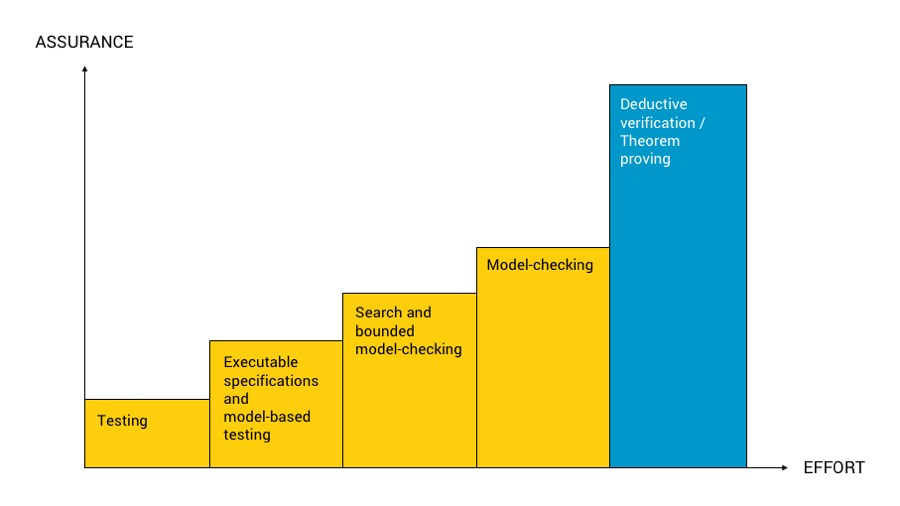
\includegraphics[width=\linewidth]{assets/verification.png}
%  \caption{Different verification methods and how they generally compare with respect to the confidence-effort trade off.}
%  \label{fig:verification}
%\end{figure}

The strongest guarantees, and thus the highest degree of trustworthiness, are obtained through deductive verification and theorem proving. In deductive verification, systems are modeled and specified inside expressive formal logical systems, and verified in a similar way to how mathematicians prove theorems - in principle by elaborating proofs of statements step-by-step. Among tools for deductive verification, \emph{proof assistants}~\cite{Geuvers2009,Harrison2014} offer the smallest trusted computing base necessary to trust verified statements, realized in modestly-sized trusted checkers that only assume a small set of axioms accepted by almost all mathematicians. Although they provide such strong guarantees, proof assistants can offer extensive automation and user support. Nevertheless, the process of figuring out what properties are relevant, how these properties are specified and building up their proofs normally requires a great deal of human ingenuity and experience. However, once everything is specified, proofs developed in proof assistants can be machine-checked, and persisted to serve as independently verifiable evidence that the properties hold for the given system~\cite{Pollack1998}.

\subsection{Coq and the Mathematical Components Library}

Coq can be viewed as consisting of, on the one hand, a small and powerful purely functional programming language, and on the other hand, a system for specifying and proving properties. A Coq user writes functions and data and then interactively constructs the proof of a theorem by trying different proof tactics that transform the state of the in-progress proof. Coq only accepts the theorem after its checker has been run on the purported proof. The Mathematical Components (MathComp) project~\cite{MathComp} provides a set of Coq libraries with standard mathematical data structures such as sequences, finite sets, and multisets, packaged to facilitate extension and formal proofs~\cite{Garillot2009}. Proofs in MathComp are written in the SSReflect proof language~\cite{Gonthier2010}, which extends Coq's proof tactic language.

%Coq has previously been used to develop a verified C compiler, formally prove mathematical results such as the four-color theorem, and verify distributed protocols (see, for example, our previous Casper formal verification effort for the Ethereum Foundation).

%We employ several existing Coq libraries which already formalized
%the majority of the mathematics we need to define and reason about Casper.
%Mathematical Components~\cite{MathComp} is a Coq library based on packaging
%mathematical structures and results in the form of Coq \emph{canonical
%  structures}, which can be reused and specialized when
%required~\cite{Garillot2009}.
%The library was used by Gonthier~et~al.\ to capture finite group theory and
%prove fundamental results in abstract algebra~\cite{Gonthier2013}.
%In addition to structures from abstract algebra, the library also contains
%encodings of and results about many standard data structures, such as numbers,
%lists, and finite sets.

\section{Formal Model and Verification Approach}
\label{sec:approach}

We model the Algorand consensus protocol in Coq as an inductive binary relation on global protocol states, and then express key properties as \emph{invariants} that hold for all protocol states that are (transitively) reachable, according to the relation, from some initial state. Ultimately, we state and prove the \emph{asynchronous safety} property of our model in this way.

Our verification approach is similar to that used for the Raft consensus protocol~\cite{Woos2016}, but is different from, for example, the approach based on reasoning on Lamport's happens-before relation used to verify the PBFT protocol~\cite{Rahli2018}. We also elide distributed separation logic, which has been used recently for consensus protocol verification in Coq~\cite{Sergey2018}.

As outlined below, our protocol model, properties, and proofs rely heavily data structures and results from the Mathematical Components project~\cite{MathComp}, and in particular its libraries for finite sets and finite maps~\cite{Cohen2019}. In total, our Coq development contains around 2000 lines of Gallina code for the specification of the model and its properties, and around 4000 lines of proof scripts that build the formal proofs.
%The source files also contain almost 1000 lines of comments that motivate and explain the specifications and lemmas.

%The modeling effort involved primarily:
%\begin{itemize}
%\item Defining all the needed data types and structures, such as message types and records, using the inductive constructions facilitated by the logic underlying Coq. Definitions were designed to utilize various existing infrastructure components, provided as Coq libraries, including most prominently the Mathematical Components (MathComp) library. These definitions specify the structure of the protocol's state.
%\item Defining both: (1) utility functions, such as computing the number of soft-votes seen by a user so far or identifying the proposal with the least credential, and (2) logical propositions asserting, for example, the preconditions for a cert-voting action or whether some event (like cert-voting) had taken place along an execution path. Functions and propositions constitute the basic building blocks using which other more complex (inductive) definitions and statements are formed.
%\item Stating and proving basic structural properties about these definitions to ensure their correctness with respect to their intended behavior, for example, showing that a defined relation is a complete order or that a function that updates user timers preserves the set of users in the system. These properties are crucial for building up other proofs of more elaborate statements. We note that definitions imported from external libraries, such as MathComp, come equipped with many useful properties already proved, which are also heavily used in our model.
%\item Formalizing the argument for safety and proving the safety theorem, which in turn required designing a proof plan and identifying the intermediate results that will need to be shown as proof obligations. This process is iterative, since many intermediate results were deep enough that they required breaking them down into smaller, more manageable pieces. The whole process was guided by the informal proof arguments documented in the protocol description by Algorand[add pointers]. We highlight some of the details of this proof later in the report.
%\end{itemize}

\subsection{Assumptions}

Most formalizations of programs and protocols are parameterized in specific ways, to be valid across a wide range of configuration choices and scenarios that may occur in practice. Our Algorand model is parameterized on a finite set of \emph{user identifiers} (e.g., names of network nodes), and on a finite set of \emph{values} used in message payloads, abstractly representing blocks and block hashes.

\begin{lstlisting}[language=Coq]
Parameters (UserId : finType) (Value : finType).
\end{lstlisting}

Values are assumed to be checkable for validity. We also consider an arbitrary, but totally ordered, datatype of credentials owned by users, and assume there is some way, given a credential, to say whether its owner is a committee member. Finally, we parameterize on delays and Algorand-specific configuration parameters such as number of votes required to move between periods. For example, these real-number parameters represent, respectively, the non-block message delivery delay, the block message delivery day, and the recovery time:
\begin{lstlisting}[language=Coq]
Parameters (lambda : R) (big_lambda : R) (L : R).
\end{lstlisting}

Besides these and other parameters (16 in total), we also express assumptions, most related to our parameters, in the form of axioms. We use four kinds of axioms:
(1) standard axioms from classical logic, (2) axioms about credentials, (3) axioms on limits of message delays, and (4) axioms on the composition of groups (quorums) of users satisfying certain conditions.

We use the first kind of axiom (three in total) to facilitate simpler use of and reasoning about real numbers.
One example of the second kind of axiom (out of two in total), expresses the uniqueness of credentials
across different users:
\begin{lstlisting}[language=Coq]
Axiom credentials_different :
 forall (u u' : UserId) (r r' p p' s s' : nat), u <> u' ->
 credential u r p s <> credential u' r' p' s'.
\end{lstlisting}
In other words, any two distinct user identifiers \lstinline{u} and \lstinline{u'} will have distinct credentials no matter what the round, period and step values are.
The two axioms of the third kind specify how the small message delivery delay \lstinline{lambda}, block message delivery delay \lstinline{big_lambda}, and the recovery time period \lstinline{L} are all related:
\begin{lstlisting}[language=Coq]
Axiom delays_order : (3 * lambda <= big_lambda < L)%R.
Axiom delays_positive : (lambda > 0)%R.
\end{lstlisting}

As one example of the fourth kind of axiom, the assumption that ``any two large-enough cert-voting committees for a given round-period-step triple must share at least one honest user'', which captures the honest supermajority assumption in Algorand for the cert-voting case, is specified as:
\begin{lstlisting}[language=Coq]
Axiom quorums_c_honest_overlap :
 quorum_honest_overlap_statement tau_c.
\end{lstlisting}
where \lstinline{quorum_honest_overlap_statement} is a definition parameterized by the committee size threshold value \lstinline{tau}:
\begin{lstlisting}[language=Coq]
Definition quorum_honest_overlap_statement (tau : nat) :=
 forall (trace : seq GState) (r p s : nat) (q1 q2:{fset UserId}),
  q1 `<=` committee r p s -> #|` q1 | >= tau ->					
  q2 `<=` committee r p s -> #|` q2 | >= tau ->					
  exists (honest_voter : UserId),
   honest_voter \in q1 /\ honest_voter \in q2 /\
   honest_during_step (r,p,s) honest_voter trace.
\end{lstlisting}
In other words, if for any two quorums of users, each of size at least \lstinline{tau}, and who are all committee members for the given \lstinline{(r,p,s)} triple, there is an honest user for the step \lstinline{(r,p,s)} who belongs to both quorums. In total, there are six axioms of this kind.

Our axioms either capture statements accepted by mathematicians (1 above) or assumptions made by Algorand designers on the runtime environment (2-4 above).

\subsection{Local and Global State}

We model local (user) state as an inductive datatype that holds information such as the current round and period, as well as blocks and votes seen during the round.

\begin{lstlisting}[language=Coq]
Record UState := mkUState {
  corrupt : bool;
  round : nat; period : nat; step : nat;
  timer : R; deadline : R; p_start : R;
  proposals     : nat -> nat -> seq PropRecord;
  stv           : nat -> option Value;
  blocks        : nat -> seq Value;
  softvotes     : nat -> nat -> seq Vote;
  certvotes     : nat -> nat -> seq Vote;
  nextvotes_open: nat -> nat -> nat -> seq UserId;
  nextvotes_val : nat -> nat -> nat -> seq Vote
}.
\end{lstlisting}

We model the global state as an inductive datatype that holds the current time, whether the network is partitioned, current state for all users, messages in transit, and received messages. In particular, the state of users in the global state is represented as a finite map from user identifier to state, and messages in transit as a finite map from user identifier to multisets of pairs of message deadlines and messages.

\begin{lstlisting}[language=Coq]
Record GState := mkGState {
  now : R;
  network_partition : bool;
  users : {fmap UserId -> UState};
  msg_in_transit : {fmap UserId -> {mset R * Msg}};
  msg_history : {mset Msg}
}.
\end{lstlisting}

\subsection{The Global Transition Relation}
The global state transition relation is defined over the \lstinline{GState} type, and denoted \lstinline{g ~~> g'} in Coq when it holds for \lstinline{g} and \lstinline{g'}. We distinguish three kinds of transitions: (a) node-internal transitions, (b) node message delivery transitions, and (c) network transitions.

Examples of the first transition (12 total) include a user proposing a block or a user certifying a block. There are eight transitions of the second form, such as a user delivering a next-vote for a block and advancing its period. The six network transitions include advancing the users' timers, entering and exiting a partition, and adversarial actions such as replaying a message.

%The global state transition relation is denoted \lstinline{g ~~> g'}, where $g$ and $g'$ are global states of the protocol. This relation defines inductively how the protocol's global state transitions into another state in one step. For example, the global state may transition into another by advancing time, having one of its users make an internal transition or by having the adversary partition the network, and so on. Each transition is guarded by certain preconditions that need to be satisfied for the transition to be enabled. Therefore, the statement that \lstinline{g ~~> g'} tells us that the preconditions for one of these global transition cases were enabled and that transition was taken to transform $g$ into $g'$.

To chain global states together, we define a \emph{trace} as a non-empty sequence of global states, where each adjacent pair belongs to the global transition relation, i.e. if state \lstinline{g$_i$} is the $i$th state in the sequence and \lstinline{g$_{i+1}$} is the $(i+1)$th state, then the pair \lstinline{g$_i$} and \lstinline{g$_{i+1}$} belongs to the global transition relation. 

By specifying path properties as propositions on traces, we are able to define generically what the property is without having to assume a fully concrete initial state. Any conditions required for the property to hold can be specified as constraints on the states of the trace being considered.

For example, the property that a block was certified in a period is captured by the following proposition:
\begin{lstlisting}[language=Coq]
Definition certified_in_period trace (r p:nat) (v:Value) :=
  exists (certvote_quorum : {fset UserId}),
  certvote_quorum `<=` committee r p 3 /\
  #|` certvote_quorum | >= tau_c /\
  forall (voter : UserId), voter \in certvote_quorum ->
   certvoted_in_path trace voter r p v.
\end{lstlisting}
It states that the proposition holds for a trace if there exists a large-enough quorum of users selected for cert-voting who actually published cert-votes along that trace for the given period (the proposition \lstinline{certvoted_in_path}).

\section{The Safety Theorem}
\label{sec:safety}

The safety theorem says that only one block may be certified in a round,
which means the blockchain will not fork.
The key assumptions of the Coq proof are some properties of cryptographic self-selection.
The cryptographic argument for the correctness of cryptographic self-selection
is given in \cite{}, but we have not formalized cryptographic reasoning so
our development takes these properties as unproved assumptions.

The statement of the theorem says that any two certificates from the same round
must be for the same block:

\begin{lstlisting}[language=Coq]
Theorem safety : forall (g0:GState) (trace:seq GState) (r:nat),
  state_before_round r g0 ->
  is_trace g0 trace ->
  forall (p1:nat) (v1:Value), certified_in_period trace r p1 v1 ->
  forall (p2:nat) (v2:Value), certified_in_period trace r p2 v2 ->
  v1 = v2.
\end{lstlisting}


Note the preconditions \lstinline{state_before_round r g0}, which states that
that initial state \lstinline{g0} is far enough back in history that no user
had yet taken any actions in round r, and \lstinline[breaklines=true]{is_trace g0 trace},
which states that the trace is a valid execution trace beginning at g0,
with all steps taken according to the global transition relation.

It is possible to end up with certificates from multiple periods of a round,
during a "network partition" which allowing the adversary to delay messages,
if cert-vote messages are delayed enough for some nodes to advance past the
period where the first certificate was produced, but these multiple certificates
will still be for the same block.

The proof of the main safety theorem[LINK safety] stated above first considers two
cases, for whether the two certificates are from the same period or different
periods.

The case when the certificates are in the same period is handled in the lemma
\lstinline{one_certificate_per_period}.
This proof uses the quorum hypotheses to conclude that there is an honest node
that contributed a cert-vote to both certificates,
and concludes by the lemma \lstinline{no_two_certvotes_in_p} which shows that an
honest node cert-votes at most once in a period (this is proved by analyzing
all transition steps an honest node can take).

The case of different periods is proved using an invariant, which is established
in the period that produces the first certificate and keeps holding for all later
periods of the same round.
The invariant property is that no step of the period produced a quorum of
open next-votes, and any quorum of value next-votes must be for a given value $v$.
This property is defined as \lstinline{period_nextvoted_exclusively_for}.

Lemma \lstinline{certificate_is_start_of_next_period} shows that this is true of
next votes from the period that produced the first certificate,
Lemma \lstinline{excl_enter_excl_next} shows that if this is true for one
period, it is true for the next.
Lemma \lstinline{prev_period_nextvotes_limits_cert_vote} shows that if the
invariant holds for one period then any certificate produced in the next period
can only be for the same value.

Most of the proofs only need the simpler quorum hypotheses that say that any
two quorums from a single step have an honest user in common.
A more complicated quorum hypothesis which relates different steps
is only needed for proving the lemma
\lstinline{certificate_is_start_of_next_period}.
The intuition is that if committee members are selected approximately randomly from
the full population of users, then any property which is true for all honest
members of one quorum must be true for most honest users in the overall population,
so any other quorum even at different steps must have at least some honest
users that also have that property.
But this isn't true if the property is that of being a committee member on
a particular step, and we don't know how to formalize the idea of a property
being unrelated to committee membership, so we assume this hypothesis only
for the specific predicate we need.

The inter-quorum hypothesis is used in between the cert-voting step and
that produced the first certificate any later next-voting steps in the same period,
with the property being whether a user had seen a quorum of soft-votes by the
time that user finished the cert-voting step.
By definition of a certificate and analysis of the transitions which send
cert-votes, this property holds for every honest user which contributed a cert-vote
to the certificate.
Then by the inter-quorum assumptions, any quorum of next-votes must include
a vote from at least one honest user which had seen a quorum of soft-votes before
making their next-vote.
By examining possible transitions this user couldn't make an open next-vote and
could only next-vote for the value which received a certificate, so the invariant
is established.

To prove the latter two lemmas \lstinline{excl_enter_excl_next} and
\lstinline{prev_period_nextvotes_limits_cert_vote} we consider that any quorum
of next-votes or cert-votes contains an honest voter, and looking at the
preconditions for an honest user to make a cert-vote or next-vote.
In either case making such a vote for a value besides $v$ or making an open
next-vote requires that the honest user had received a quorum of
soft-votes for another value or a quorum of open next-votes from the
previous period.
The latter is ruled out because the invariant says no such quorum of votes
was sent, and lemma \lstinline{no_bottom_quorums_during_from_nextvoted_excl}
contains the argument that therefore no such quorum of votes could
be received.
Lemma \lstinline{no_bottom_quorums_during_from_nextvoted_excl}
states that any quorum of soft-votes must be votes for value $v$ if the
invariant for value $v$ held in the previous period.
It is proved by analyzing the transitions which move a user to a new period
to show that all honest users get $v$ as their ``starting value'',
and analyzing the transitions which send soft-votes to show that this
starting value and the absence of quorums of open next-votes means any honest
soft-vote can only be for value $v$.

By the overall inductive argument, we then have the safety theorem that the
protocol cannot fork.
\section{Conclusion}
\label{sec:conclusion}

In this project, we successfully completed a complete model of the Algorand consensus protocol in Coq. In doing so, we mechanically verified the asynchronous safety theorem, a key claim of the Algorand protocol, while also outlining the precise assumptions under which the safety theorem holds. Proving this (along with the vast majority of lemmas proved leading to asynchronous safety) gives assurance to the security of the Algorand protocol, which is extremely important for blockchain protocols with potentially billions of dollars at stake.

Concerning future efforts, the model we developed as part of this effort is generic, in that it captures the dynamics of the Algorand consensus protocol in a way that is orthogonal to the properties that we verify about it. This means that the model can be readily used to verify other properties of the system beyond asynchronous safety, including most importantly liveness. In fact, we anticipate that many of the smaller results shown about the protocol and used in the proof of safety will also constitute essential ingredients of the liveness proving effort. Nevertheless, proving liveness will probably require showing additional results, especially those related to timely message delivery and network partitioning, some of which were not needed for the safety argument. But the model already has these components (time, message delays and network partitioning) and going into investigating liveness (and perhaps other properties) will be a seamless continuation of the effort involved in this project.


%% Acknowledgments
\begin{acks}

We thank Jing Chen, Nickolai Zeldovich, and Victor Luchangco from Algorand for their help throughout the project. This work was funded by Algorand.

%% contents suppressed with 'anonymous'
%  %% Commands \grantsponsor{<sponsorID>}{<name>}{<url>} and
%  %% \grantnum[<url>]{<sponsorID>}{<number>} should be used to
%  %% acknowledge financial support and will be used by metadata
%  %% extraction tools.
%  This material is based upon work supported by the
%  \grantsponsor{GS100000001}{National Science
%    Foundation}{http://dx.doi.org/10.13039/100000001} under Grant
%  No.~\grantnum{GS100000001}{nnnnnnn} and Grant
%  No.~\grantnum{GS100000001}{mmmmmmm}.  Any opinions, findings, and
%  conclusions or recommendations expressed in this material are those
%  of the author and do not necessarily reflect the views of the
%  National Science Foundation.
\end{acks}

\balance

%% Bibliography
\bibliography{bib}



%% Appendix
%\appendix
%\section{Appendix}
%
%Text of appendix \ldots

\end{document}
